\documentclass[tikz,border=5pt]{standalone}
\usepackage{tikz}
\usepackage{amsmath}
\usetikzlibrary{arrows.meta,positioning}
\definecolor{nebula}{HTML}{6366F1}
\definecolor{spark}{HTML}{14B8A6}
\definecolor{ink}{HTML}{334155}
\begin{document}
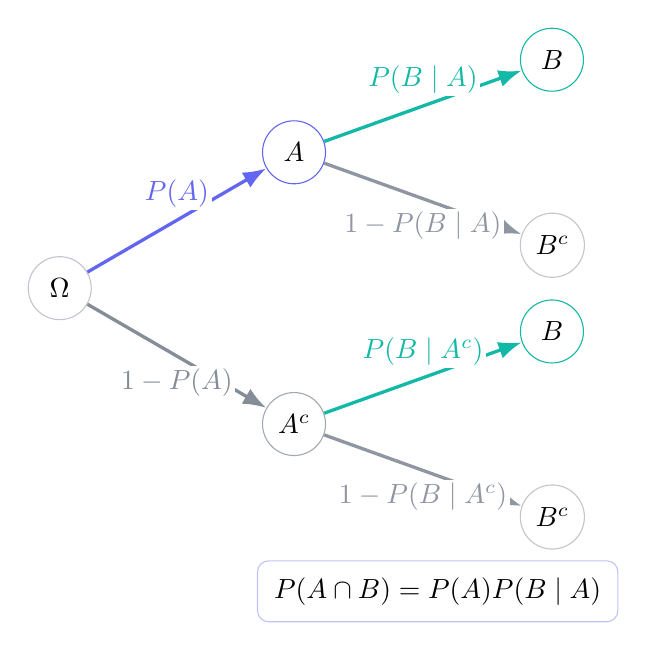
\begin{tikzpicture}[font=\sffamily,>=Latex]
  \tikzset{event/.style={draw=ink!30,circle,fill=white,minimum size=8mm}}
  \node[event] (start) {$\Omega$};
  \node[event,above right=1.15cm and 2.4cm of start,draw=nebula] (a) {$A$};
  \node[event,below right=1.15cm and 2.4cm of start,draw=ink!45] (na) {$A^c$};
  \node[event,above right=.6cm and 2.7cm of a,draw=spark] (ab) {$B$};
  \node[event,below right=.6cm and 2.7cm of a] (anb) {$B^c$};
  \node[event,above right=.6cm and 2.7cm of na,draw=spark] (nab) {$B$};
  \node[event,below right=.6cm and 2.7cm of na] (nanb) {$B^c$};
  \draw[->,very thick,nebula] (start)--(a) node[midway,above=3pt,fill=white,inner sep=1pt] {$P(A)$};
  \draw[->,very thick,ink!60] (start)--(na) node[midway,below=3pt,fill=white,inner sep=1pt] {$1-P(A)$};
  \draw[->,very thick,spark] (a)--(ab) node[midway,above=3pt,fill=white,inner sep=1pt] {$P(B\mid A)$};
  \draw[->,very thick,ink!55] (a)--(anb) node[midway,below=3pt,fill=white,inner sep=1pt] {$1-P(B\mid A)$};
  \draw[->,very thick,spark] (na)--(nab) node[midway,above=3pt,fill=white,inner sep=1pt] {$P(B\mid A^c)$};
  \draw[->,very thick,ink!55] (na)--(nanb) node[midway,below=3pt,fill=white,inner sep=1pt] {$1-P(B\mid A^c)$};
  \node[draw=nebula!40,rounded corners=4pt,fill=white,inner sep=6pt] at (4.8,-3.85)
    {$P(A\cap B)=P(A)P(B\mid A)$};
\end{tikzpicture}
\end{document}
